% !Mode:: "TeX:UTF-8"


%-------------------------------------------------------------------------------
% This file provides a skeleton ATLAS document.
%-------------------------------------------------------------------------------
% \pdfoutput=1
% The \pdfoutput command is needed by arXiv/JHEP/JINST to ensure use of pdflatex.
% It should be included in the first 5 lines of the file.
%-------------------------------------------------------------------------------
% Specify where ATLAS LaTeX style files can be found.


%maybe uncomment:\newcommand*{\ATLASLATEXPATH}{latex/}

% Use this variant if the files are in a central location, e.g. $HOME/texmf.
% \newcommand*{\ATLASLATEXPATH}{}



%-------------------------------------------------------------------------------
%\documentclass[UKenglish,texlive=2013,PAPER,coverpage]{\ATLASLATEXPATH atlasdoc}
\documentclass[
dissertation,
copyright,
final,
justified,
numbers,
sort&compress,
numsections,
gsmodern,
]{uothesis}

% The language of the document must be set: usually UKenglish or USenglish.
% british and american also work!
% Commonly used options:
%  texlive=YYYY          Specify TeX Live version (2013 is default).
%  atlasstyle=true|false Use ATLAS style for document (default).
%  coverpage             Create ATLAS draft cover page for collaboration circulation.
%                        See atlas-draft-cover.tex for a list of variables that should be defined.
%  cernpreprint          Create front page for a CERN preprint.
%                        See atlas-preprint-cover.tex for a list of variables that should be defined.
%  PAPER                 The document is an ATLAS paper (draft).
%  CONF                  The document is a CONF note (draft).
%  PUB                   The document is a PUB note (draft).
%  txfonts=true|false    Use txfonts rather than the default newtx - needed for arXiv submission.
%  paper=a4|letter       Set paper size to A4 (default) or letter.

%-------------------------------------------------------------------------------
% Extra packages:
%\usepackage{\ATLASLATEXPATH atlaspackage}
% Commonly used options:
%  biblatex=true|false   Use biblatex (default) or bibtex for the bibliography.
%  backend=biber         Use the biber backend rather than bibtex.
%  subfigure|subfig|subcaption  to use one of these packages for figures in figures.
%  minimal               Minimal set of packages.
%  default               Standard set of packages.
%  full                  Full set of packages.
%-------------------------------------------------------------------------------
% Style file with biblatex options for ATLAS documents.
%\usepackage{\ATLASLATEXPATH atlasbiblatex}

% Package for creating list of authors and contributors to the analysis.
%\usepackage{\ATLASLATEXPATH atlascontribute}

% Useful macros
%\usepackage{\ATLASLATEXPATH atlasphysics}

% See doc/atlas-physics.pdf for a list of the defined symbols.
% Default options are:
%   true:  journal, misc, particle, unit, xref
%   false: BSM, hion, math, process, other, texmf
% See the package for details on the options.
%\setcounter{secnumdepth}{3}% This is supposed to change the depth of references (default 2)
\usepackage{graphicx}

\usepackage{atlasphysics}

\usepackage{float}
%\usepackage{floatrow}
%\floatsetup[table]{capposition=top}
\usepackage{tabularx}
\usepackage{pdflscape}
\usepackage{siunitx}
\usepackage{footnote}
\usepackage{footnotebackref}
\usepackage{tocbibind}
\usepackage{enumitem}

\usepackage{epsfig}
\usepackage{epstopdf}
%\usepackage{subcaption}
%\usepackage{caption}

\usepackage{enumerate}
\usepackage{rotating} %GR added
%\usepackage{mdwlist}
\usepackage{multirow}
\usepackage{multicol}
\usepackage{pdflscape}
\usepackage{longtable}
\usepackage{slashed}
\usepackage{verbatim}
\usepackage{hyperref} %If you get an error due to hyperref package, delete your old INT.aux file then recompile.
\usepackage{tikz}
\usepackage[compat=1.1.0]{tikz-feynman}
%\usepackage{multirow}
\usepackage{slashed}
\usepackage{smartdiagram}

\usepackage{booktabs} %Use for smarter Tables
\usepackage{pifont}
\usepackage{tabu}
\usepackage{amsmath}
\usepackage{slashed}
\usepackage{color}
\usepackage{placeins}
\usepackage{xspace}
\usepackage{adjustbox}
\usepackage{dcolumn}
\usepackage[flushleft]{threeparttable}
%\usepackage{feynmp}

\usepackage[style=numeric-comp,backend=biber,sorting=none]{biblatex}
%\usepackage[hang,center]{subfigure}
%\usepackage{subfigure}

%\captionsetup[figure]{labelformat=parens, labelsep=newline}

% set up labelformat and labelsep for subfigure

\captionsetup[subfigure]{labelformat=simple}%, labelsep=period}%, labelsep=colon}
 


%\usepackage[utf8]{inputenc}

% Files with references for use with biblatex.
% Note that biber gives an error if it finds empty bib files.

\addbibresource{thesis.bib}

%\addbibresource{bibtex/bib/ATLAS.bib}
%\bibliography{thesis.bib}
%% Paths for figures - do not forget the / at the end of the directory name.
\graphicspath{{logos/}{figures/}}

% Add you own definitions here (file atlas-document-defs.sty).
%\usepackage{atlas-document-defs}

%-------------------------------------------------------------------------------
% Generic document information
%-------------------------------------------------------------------------------

%% Title, abstract and document 
%\input{atlas-document-metadata}

%% Author and title for the PDF file
\hypersetup{pdftitle={ATLAS document},pdfauthor={The ATLAS Collaboration}}

%-------------------------------------------------------------------------------
% Content
%-------------------------------------------------------------------------------
\newcommand{\Lagr}{\mathcal{L}}
%\setlength\parindent{0pt}
\newcommand{\apkg}[2]{\href{#1}{\texttt{#2}}}


\usepackage{lineno, lipsum}
%\RequirePackage{lineno}
%\linenumbers


\begin{document}
\renewcommand\texteuro{FIXME} 
%\begin{linenumbers}
\begin{runninglinenumbers}

%\thispagestyle{empty}
\begin{center}
SEARCH FOR HIGGS BOSON PAIR PRODUCTION IN THE FULLY BOOSTED ${b\overline{b}WW\text{*}}$ CHANNEL IN ${\sqrt{s}}$ =  13 TeV PROTON-PROTON COLLISIONS AT THE LARGE HADRON COLLIDER USING THE ATLAS DETECTOR

\vspace*{\fill}
by\\
JOHN CHRISTOPHER STEPHEN MYERS
\vspace*{\fill}

A DISSERTATION \\
Presented to the Department of Physics and the Graduate Scool of the University of Oregon in partial fulfillment of the requirements for the degree of Doctor of Philosophy\\~\\
March 2019
\end{center}
%\abstract{
This dissertation presents a search for double Higgs production in the ${b\bar{b}WW^{*}}$ final state in proton-proton collisions at the ATLAS detector at the Large Hadron Collider. Double Higgs production is predicted in the Standard Model with a cross section of ${\sigma_{HH} = 33.53^{+4.3\%}_{-6.0\%}\pm{5.9\%}}$ fb. Many Beyond the Standard Model theories predict enhancements to the production cross section through resonant production. 
\indent The 2015-2016 ATLAS dataset has an integrated luminosity of 36.1 fb\textsuperscript{-1} with a center of mass energy of ${\sqrt{s} = 13 TeV}$. Candidate events are broken into two kinematic regions: a resolved selection containing one lepton (either an electron or muon), 2 b-tagged calorimeter jets, 2 light-flavor jets, and missing transverse energy; and a boosted analysis containing one lepton (electron or muon), two large radius jets, one with two ghost associated, b-tagged track-jets and missing transverse energy. No significant deviation from background was observed a cross section upper limit was set for the SM double Higgs production of 10 pb and for resonant production as a function of HH invariant mass from 500 GeV to 3000 GeV.
}
%\school{University of Oregon, Eugene, Oregon}%Graduate school
\school{The Ohio State University, Columbus, Ohio}%Undergraduate school

\degree{Doctor of Philosophy, Physics, 2018 University of Oregon}
\degree{Bachelor of Science, Physics, 2013, The Ohio State University}


%%There is a known issue if you do not fill in the interests section.  If you want to skip this section, comment out line#526 of uothesis.cls file \cvitem{GRANTS, AWARDS AND HONORS}{\@awards}
\interests{Boosted object reconstruction}
\interests{Trigger and detector operations}

\position{Graduate Research Assistant, University Of Oregon: ATLAS Collaboration, 2015-Present}%Your job while at UO, probably graduate research assistant.
\position{Graduate Teaching Assistant, University Of Oregon: Department of Physics, 2013-2015}

\award{}%If you didn't get any awards you'll have to comment out things in the uothesis. I dug up something from my undergraduate
\publication{List of publications with significant contributions:}
\publication{\fullcite{Aaboud2019}}
\publication{Co-authored on 124 publications with minor contributions can be found at Inspire (search parameters: exactauthor:John.Myers.1)}
%Fill this out with your publications.

%\input{acknowledgements}
%\maketitle
%\tableofcontents
%%%%%Use this as a filler to get the template working
%%Introduction
\chapter{Introduction}
The Standard Model (SM) is the culmination of more than a century of work. The first piece added to the puzzle was the electron, discovered in 1891. Since then, 24 other particles have been discovered, with the final piece, the Higgs Boson, being added in 2012. Since it was theorized, the SM has held up to rigorous experimentation and remains an unbeaten theory of fundamental matter and forces. Even though the SM is widely successful, it fails to explain all observed phenomena. Gravity, neutrino masses, dark matter, along with other observations, all lacking explanation within the SM. The remaining task is to probe the extremes of the SM to either more precisely measure the parameters or to find its limit.
%Include this is a search for BSM production
\section{The Standard Model}
The Standard Model defines the basic building blocks of matter and force and the interactions between them. Normal matter that we interact with on a daily basis is made of protons, neutrons, and electrons. Electrons are a fundamental particle, called a lepton, meaning they are not made of smaller constituents. However, protons and neutrons are not fundamental particles. They are a composite of up and down quarks, two more fundamental particles. The protons are made of 2 ups and a down and the neutrons are made of two downs and an up. Leptons and quarks are both different types of fermions. \linebreak
\indent Fermions are spin-${\frac{1}{2}}$ particles that make up all matter in the SM. The fermions can be broken down into 3 "generations". Where a generation contains two quarks, one with electric charge ${+\frac{2}{3}}$ and one with electric charge ${-\frac{1}{3}}$, one electrically charged lepton, charge -1, and one electrically neutral lepton. The quarks have an additional color charge, of which there are 3 charges. This is additional quantum number associated with the strong force. In all, this gives 12 fermions. \linebreak 

\begin{table}[h]
\begin{center}
\footnotesize
\begin{tabular}[h]{|c||c|c|c|c|}
\hline
 & Particle & Spin & Charge & Mass \\
\hline\hline
Quarks &&&&\\
\hline
u type &u& & &${2.4^{+0.6}_{-0.4} MeV}$\\
 &c&${\frac{1}{2}}$&${\frac{2}{3}}$&${1.28\pm{0.03} GeV}$\\
 &t& & &${173.1\pm{0.6} GeV}$\\
\hline
d type & d& & & ${4.7^{+0.5}_{-0.4} MeV}$\\
 & s & ${\frac{1}{2}}$ & ${-\frac{1}{3}}$ & ${96^{+8}_{-4} MeV}$\\
 & b & & & ${4.18^{+0.04}_{-0.03} GeV}$\\
\hline\hline
Leptons &&&&\\
\hline
e family & e & ${\frac{1}{2}}$ & -1 &${0.5109989461\pm{}0.000000003 MeV}$\\
 & ${\nu_{e}}$ & & 0 & ${< 2 eV}$\\
 \hline
${\mu}$ family & ${\mu}$ & ${\frac{1}{2}}$ & -1 &${105.6583745\pm{}0.0000024 MeV}$\\
 & ${\nu_{\mu}}$ & & 0 & ${< 2 eV}$\\
 \hline
${\tau}$ family & ${\tau}$ & ${\frac{1}{2}}$ & -1 &${1776.86\pm{}0.12 GeV}$\\
 & ${\nu_{\tau}}$ & & 0 & ${< 2 eV}$\\
 \hline\hline
 Bosons &&&&\\
 \hline
 Vector & ${\gamma}$ & 1 & 0 & ${< 10^{-18} eV}$\\
 & ${g}$ & 1 & 0 & ${0}$\\
 & ${W}$ & 1 & ${\pm}$ & ${80.385\pm{}0.0015 GeV}$\\
 & ${Z}$ & 1 & 0 & ${91.1876\pm{}0.0021 GeV}$\\
 \hline
 Scalar & H & 0& 0 & ${125.09\pm{}0.21\pm{}0.11 GeV}$\\
 \hline
\end{tabular}
\caption{Particles of the Standard Model (ref XXX (ian or PDG))}
\label{tab:SM}
\end{center}
\end{table}

\indent Gauge bosons are spin-${1}$ particles responsible for carrying the fundamental forces in the standard model. There are 12 physical gauge boson. The photon ${\gamma}$ is a massless, charge neutral force carrier for the electromagnetic force. The nuclear forces are carried by 3 massive gauge bosons. A chargeless Z boson and two charged W bosons, ${Q = \pm 1}$. Together, these 4 bosons control the electroweak interactions in the standard model. The remaining 8 bosons are the gluons, the force carriers for the strong nuclear interaction. Gluons are massless, electrically neutral particles that have two color charges. There is a gluon for each combination of the three color charges, giving the 8 total gluons. \linebreak
\indent The remaining piece of the standard is the Higgs Boson. The Higgs boson is a massive Scalar, spin-${0}$, chargeless boson. The Higgs boson is responsible for giving mass to the massive electoweak bosons through electroweak symmetry breaking. The particles and their properties are in Table ~\ref{tab:SM}\linebreak
\subsection{Interactions}
The SM is governed by three different types of interactions. For leptons, the overarching theory is quantum electrodynamics (QED). QED describes how particles behave under electroweak interactions. This can be broken down further into the electromagnetic interaction and the weak interaction. The electromagnetic interaction defines the interaction of electrically charged particles with photons. The fundamental diagram for the electromagnetic interaction is electron-positron annihilation ~\ref{Fey:e-p}. Where an electron and a positron collide and produce two photons. This can also be reversed, two photons interact and produce an electron-positron pair. The strength of this interaction is the electrical charge e. \linebreak

\begin{figure}[h]

\begin{center}
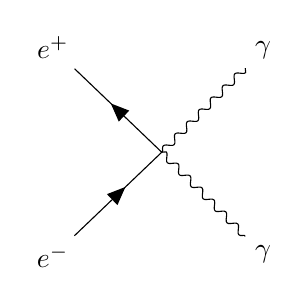
\begin{tikzpicture}
\begin{feynman}
\vertex (c) ;
\vertex [below left =of c] (i1){\(e^{-}\)};
\vertex [above left=of c] (i2) {\(e^{+}\)};
\vertex [below right=of c] (f1){\(\gamma\)};
\vertex [above right= of c] (f2){\(\gamma\)};
\diagram* {
(i1) -- [fermion] (c) -- [fermion] (i2) ,
(f1) -- [photon] (c)-- [photon] (f2)
};
\end{feynman}
\end{tikzpicture}
\caption{Electron-Positron Annihilation}
\label{Fey:e-p}
\end{center}
\end{figure}

\indent The weak interaction defines the interaction of particles under the weak isospin quantum number. There are two copies of each of every fermion, a left and a right-handed chirality version. Particle with a right-handed chirality have a weak isospin T = 0. These particles exist as singlets and do not interact with the weak force. Left-handed particles have a weak isospin T =  ${\frac{1}{2}}$. These particles live as doublets as illustrated in table ~\ref{tab:chiral}. For these particles, the third component of the weak isospin T\textsubscript{3}, ${+\frac{1}{2}}$ for up-type quarks and charged leptons and ${-\frac{1}{2}}$ for down-type quarks and neutral leptons. Under weak interactions, particles with ${T_{3} = +\frac{1}{2}}$ always transform into particles with ${T_{3} = -\frac{1}{2}}$, or vice versa.\linebreak

\begin{table}[h]
\begin{center}
\def\arraystretch{1.5}
\begin{tabular}[h]{|c|c|}
\hline
Left Handed Fermions, ${T = \frac{1}{2}, T_{3} = \pm\frac{1}{2}}$ & Right Handed Fermions, ${T = 0, T_{3} = 0}$\\
\hline\hline
${\binom{u}{d}}$, ${\binom{c}{s}}$, ${\binom{t}{b}}$, ${\binom{e}{\nu_{e}}}$, ${\binom{\mu}{\nu_{\mu}}}$, ${\binom{\tau}{\nu_{\tau}}}$ & u, d, c, s, t, b, e, ${\nu_{e}}$, ${\mu}$, ${\nu_{\mu}}$, ${\tau}$, ${\nu_{\tau}}$ \\
\hline
\end{tabular}
\caption{Particles of the Standard Model (ref XXX (ian or PDG))}
\label{tab:chiral}
\end{center}
\end{table}


 \indent The remaining piece of the weak interaction is the W boson. The W has an isospin of T = 1. This gives three option for the third component of isospin, ${T_{3} = +1, 0, -1}$ which give the W\textsuperscript{+}, the W\textsuperscript{0}, and the W\textsuperscript{-}. W\textsuperscript{0} will be discussed more in ~\ref{ssec:Higgs}. The ${W^{\pm}}$ either raise or lower the ${T_{3}}$ of the fermions. ~\ref{Fig:weak_dia} is an example of a weak interaction.\linebreak

\begin{figure}[h]
\begin{center}

\begin{tikzpicture}
\begin{feynman}
\vertex (i1){\(e^{-}\)};
\vertex [right =of i1] (c);
\vertex [right=of c] (f1) {\(\nu_{e}\)};
\vertex [below right=of c] (f2){\(W^{-}\)};
\diagram* {
(i1) -- [fermion] (c),
(f2) -- [boson] (c)-- [fermion] (f1)
};
\end{feynman}
\end{tikzpicture}
\caption{electron emitting an electron neutrino and a W Boson}
\label{Fig:weak_dia}
\end{center}
\end{figure}

%Here, write about mixing and electroweak interaction?
%Also need to talk briefly about QCD
%Need to talk about b-quarks specifically.

%\begin{equation}
%Y_{W} = 2(Q - T_{3})
%\end{equation}


\indent %Need to talk about couplings and decays more in depth here
\subsection{The Higgs Mechanism and Higgs Boson}
\label{ssec:Higgs}
%Start with need massless gauge bosons to fufill local gauge invariance. So we have W 1,2,3, and b. explain the mixing and the  break the symmetry to give the W+- Z and photon. Give math to explain this?? Show how this gives rise to a new boson, the higgs. 
QED is a gauge invariant theory. This means the Lagrangian that describes the system is invariant under local gauge transformations. For the electroweak theory, this is the electroweak symmetry. To satisfy this symmetry, the bosons must be massless. However, the electroweak bosons in the standard model, the ${W^{\pm}}$ the ${Z}$ and the ${\gamma}$ are not all massless. This means that the electroweak symmetry must be broken by something.\linebreak

\begin{figure}[h]
\begin{center}
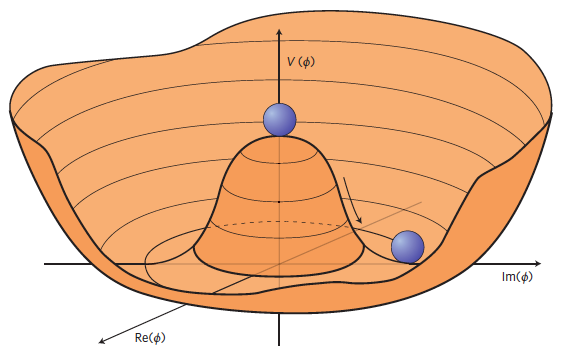
\includegraphics[scale=0.65]{figures/higgspotential}
\caption{The Higgs potential (from http://cds.cern.ch/record/1638469/plots) }
\label{Fig:higgspot}
\end{center}
\end{figure}

\indent In QED, the five gauge bosons are ${W^{i}_{\mu}, i = 1,2,3}$ and ${B_{\mu}}$. These bosons couple to a complex scalar Higgs doublet, ${\Phi \equiv \binom{\phi^{+}}{\phi^{0}}}$. This doublet has a scalar potential.
\begin{equation}
V(\Phi) = \mu^{2}|\Phi^{\dagger}\Phi| + \lambda(|\Phi^{\dagger}\Phi|)^{2}
\end{equation}
Where ${\mu^{2} < 0}$. This gives the Mexican hat shaped potential seen in figure ~\ref{Fig:higgspot}, with a minimum energy at 
\begin{equation}
\langle \phi \rangle = \sqrt{-\frac{\mu^{2}}{2\lambda}}\equiv \frac{\nu}{\sqrt{2}}
\end{equation}
called the vacuum expectation value (VEV) of ${\phi}$. The choice of the direction of fluctuation is arbitrary but can be chosen such that


 
\begin{equation}
\phi_{0} = \frac{1}{\sqrt{2}} \binom{0}{\nu}
\end{equation}
After the direction is chosen and the only remaining piece is the scalar field h(x), giving 
\begin{equation}
\phi(x) = \phi_{0} + h(x)
\end{equation}
The doublet can now be described by 
\begin{equation}
\Phi = \frac{1}{sqrt{2}} \binom{0}{v+h(x)}
\end{equation}
The Higgs field couples to the gauge bosons as 
\begin{equation}
(\frac{g}{2}\overrightarrow{\tau}\cdot \overrightarrow{W} + \frac{g'}{2}B)\phi_{0}
\end{equation}
Where ${\overrightarrow{\tau}}$ are the Pauli matrices, ${\overrightarrow{W}}$ are ${W_{1,2,3}}$ and g, g' are the coupling constants. The result of the coupling is the acquisition of mass by three eigenstates of the bosons, 
\begin{equation}
\begin{split}
W^{\pm} = \frac{1}{\sqrt{2}}(W^{1}_{\mu} \mp iW^{2}_{\mu})\\
Z^{\mu} = \frac{-g'B_{\mu} + gW^{3}_{\mu}}{\sqrt{g^{2} + g'^{2}}}\\
A^{\mu} = \frac{gB_{\mu} + g'W^{3}_{\mu}}{\sqrt{g^{2} + g'^{2}}}
\end{split}
\end{equation}
These four eigenstates are the bosons we observe in the standard model. With Masses
\begin{equation}
\begin{split}
M^{2}_{W} = \frac{1}{4}g^{2}\nu^{2} \\
M^{2}_{Z} = \frac{1}{4}(g^{2} + g'^{2})\nu^{2} \\
M_{A} = 0
\end{split}
\end{equation}
Through the mixing that occurs in the spontaneous electroweak symmetry breaking gives mass to the standard model Gauge Bosons while leaving the photon massless. However, for this to occur, an additional scalar field, the Higgs Field, is required.\linebreak
\indent The Higgs Boson is an excitation in the scalar Higgs field predicted in 1964. The decay mechanism of this massive boson was predicted by Peter Higgs, allowing for the decay products to be measured. Giving a way to prove the existence of the scalar Higgs field. In 2012, a Higgs like scalar boson was discovered at the LHC by the ATLAS and CMS experiments with a mass of 125GeV/c\textsuperscript{2} (ref XXX https://arxiv.org/abs/1207.7214). Since the discovery, many measurements have been made of this Higgs Boson to compare it to the standard model Higgs Boson. So far, the Higgs Boson has held up to these tests. The Higgs Boson has spin-parity J\textsuperscript{P} = 0\textsuperscript{+} 
(ref XXX %https://www.sciencedirect.com/science/article/pii/S0370269313006527?via%3Dihub)
, decays to bb (https://www.sciencedirect.com/science/article/pii/S0370269318307056), ${\gamma\gamma, \tau\tau}$,(ref XXX https://arxiv.org/abs/1811.08856) WW and ZZ have been measured with appropriate signal strengths, and no significant deviations have been observed in any Run 2 analyses. However, there are still many parameters of the Higgs Boson that still need measured. One of which is the triple Higgs coupling.
%Do I want to include more about the higgs discovery. 

%%%%%Use this as a filler to get the template working
%%Introduction
\chapter{Di-Higgs Production}
\label{chap:dihiggs}
Measuring di-Higgs production is necessary to further confirm the SM or find evidence for beyond the SM physics. The small SM production rate makes the channel an important place to look for new physics.  In particular, the di-Higgs production rate gives a handle to more accurately measure the Higgs potential.  This dissertation looks at both the measurement of the SM di-Higgs production rate and to search for new physics through resonant di-Higgs production. 
\section{Standard Model}
The Higgs self coupling potential in the SM is
\begin{equation}
V_{\mathrm{self-coupling}} = \lambda(|\Phi^{\dagger}\Phi|)^{2}
\end{equation}
When ${\Phi}$ is expanded around the VeV, $v$, the self coupling term can be written as
\begin{equation}
V_{\mathrm{self-coupling}} \supset \lambda v H^{3} + \frac{\lambda}{4}H^{4}
\end{equation}
where the first term, ${\lambda v H^{3}}$ is the coupling between three Higgs bosons with strength ${\lambda v \equiv \lambda_{HHH}}$\cite{Belusevic:2004pz}. The trilinear Higgs coupling can be probed at the LHC by measuring the cross section of events with two Higgs Bosons in the final state.\newline



\indent  Currently at the LHC, there are two dominant ways to produce di-Higgs events, the trilinear Higgs coupling gluon-gluon fusion (ggF) diagram and a box diagram, figure ~\ref{fig:dihiggs}. These diagrams interfere destructively, resulting in a SM prediction for the cross section, 
\begin{equation}
\sigma_{\mathrm{HH}} = 33.53\mathrm{fb}^{+4.3\%}_{-6.0\%}(\mathrm{QCD \ unc.})\pm{5.9\%} \mathrm{(other \ unc.)} 
\end{equation}
in pp collisions at 13 TeV \cite{Sirunyan:2018two}. This makes the trilinear coupling extremely hard to measure at the LHC. Additionally, since the cross section is so small, it is an promising place to look for deviations from the SM, since any enhancement to the cross section would be indicative of new physics.

\begin{figure}[h]
\footnotesize
\begin{center}
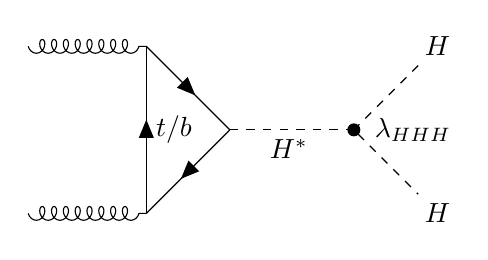
\begin{tikzpicture}
\begin{feynman}
\vertex (i1);
\vertex [right = of i1] (t1);
\vertex [dot][below right =of t1] (t3);
\vertex [below left= of t3] (t2);
\vertex [left = of t2] (i2);
\vertex [right =of t3][dot](h){};
\vertex [above right = of h] (f1){\(H\)};
\vertex [below right = of h] (f2){\(H\)};
\diagram* {
(i1) -- [gluon] (t1),
(i2) -- [gluon] (t2),
(t1) -- [fermion](t3) -- [fermion] (t2) -- [fermion,edge label'=\(t/b\)](t1),
(t3) -- [scalar,edge label'=\(H^{*}\)] (h),
(f1) -- [scalar] (h) -- [scalar](f2)
};
\vertex [right=0.75cm of h] {\(\lambda_{HHH}\)};
\end{feynman}
\end{tikzpicture}
\hspace{1cm}
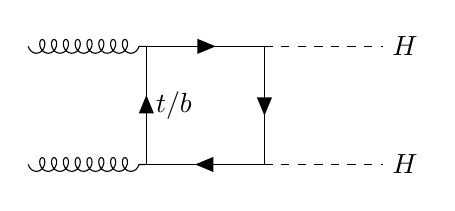
\begin{tikzpicture}
\begin{feynman}
\vertex (i1);
\vertex [ right = of i1] (t1);
\vertex [right = of t1] (t2);
\vertex [below = of t2] (t3);
\vertex [left = of t3] (t4);
\vertex [ left=of t4] (i2);
\vertex [ right =of t2] (f1){\(H\)};
\vertex [ right=of t3] (f2){\(H\)};
\diagram* {
(i1) -- [gluon] (t1),
(i2) -- [gluon] (t4),
(t1) -- [fermion](t2) -- [fermion] (t3) -- [fermion](t4) -- [fermion,edge label'=\(t/b\)] (t1),
(t2) -- [scalar] (f1),
(t3) -- [scalar] (f2)
};
\end{feynman}
\end{tikzpicture}
\caption[Di-Higgs production diagrams]{The dominate production method for di-Higgs events at the LHC with ${\sqrt{s} = 13 \text{ TeV}}$, with the trilinear Higgs coupling on the left}
\end{center}
\end{figure}
\label{fig:dihiggs}

\indent The SM di-Higgs production is a continuum production, with a turn-on at two times the Higgs mass, 250 GeV. Figure ~\ref{fig:SM_cont} shows the continuum distribution, as expected, it is a falling power law distribution peaked around 400 GeV. 

\begin{figure}[h]
\begin{center}
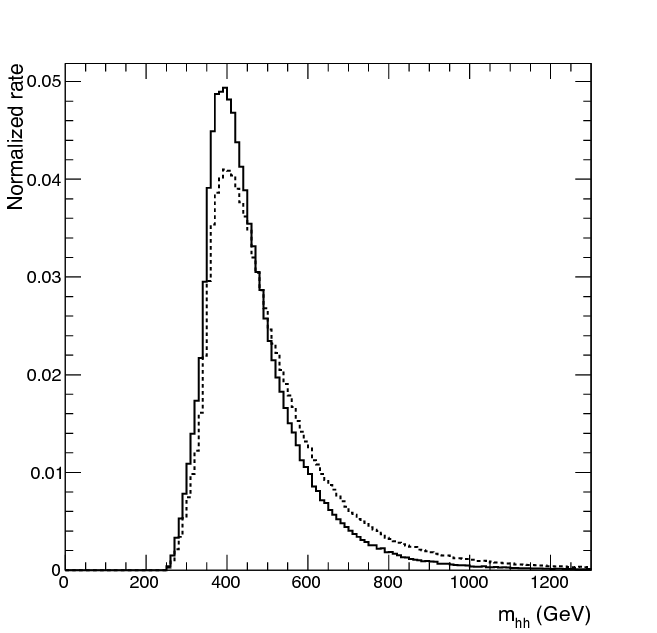
\includegraphics[scale=0.3]{figures/SM_continuum}
\caption[Normalized di-Higgs cross section]{Normalized differential cross section for pp ${\rightarrow}$ hh in the SM as a function of the invariant mass of the two Higgs bosons. The solid and dotted lines correspond respectively to ${\sqrt{s} = 14 \text{ and } 100 \text{ TeV}}$ .\cite{azatov:2015}}
\label{fig:SM_cont}
\end{center}
\end{figure}


\section{Resonant Production}
There are several BSM models that may enhance the rate of di-Higgs production at the LHC. This section will give an overview of a few of these models
\subsection{Complex Higgs Singlet}
The addition of a complex scalar singlet to the SM results in three neutral scalar particles after spontaneous symmetry breaking, which mix to give mass eigenstates, including the observed 125 GeV scalar \cite{PhysRevD.97.015022}.\newline
The normalizable scalar potential is
\begin{equation}
\begin{split}
V(\Phi,S_{c}) = \frac{\mu^{2}}{2}\Phi^{\dagger}\Phi + \frac{\lambda}{4}(\Phi^{\dagger}\Phi)^{2} \\
+ (\frac{1}{4}\delta_{1}\Phi^{\dagger}\Phi{}S_{c} + \frac{1}{4}\delta_{3}\Phi^{\dagger}\Phi{}S_{c}^{2} \\
+ a_{1}S_{c} + \frac{1}{4}b_{1}S_{c}^{2} + \frac{1}{6}e_{1}S_{c}^{3} + \frac{1}{6}e_{2}S_{c}|S_{c}|^{2} \\
+ \frac{1}{8}d_{1}S^{4} + \frac{1}{8}d_{3}S_{c}^{2}|S_{c}|^{2} + \mathrm{H.C.}) \\
+ \frac{1}{4}d_{2}(|S_{2}|^{2})^{2} + \frac{\delta_{2}}{2}\Phi^{\dagger}\Phi|S_{c}|^{2} + \frac{1}{2}b_{2}|S_{c}|^{2}
\end{split}
\end{equation}
\indent After spontaneous symmetry breaking, the fields are defined as:
\begin{equation}
\Phi = \binom{0}{\frac{h+v}{\sqrt{2}}}; S_{c} = \frac{1}{\sqrt{2}}(S+v_{s} + i(A + v_{A})).
\end{equation}
$v_{A}$ is set to 0 to conserve CP symmetry.\newline
The mass eigenstate fields are given by:
\begin{equation}
\begin{pmatrix}
h_{1}\\
h_{2}\\
h_{3}
\end{pmatrix}
= \begin{pmatrix}
c_{1} & -s_{1} & 0\\
s_{1}c_{2} & c_{1}c_{2} & s_{2}\\
s_{1}s_{2} & c_{1}s_{2} & -c_{2}
\end{pmatrix} 
\begin{pmatrix}
h\\
S\\
A\\
\end{pmatrix}
\end{equation}
where ${c_{i} = \cos{\theta_{i}}}$, h is the SU(2) doublet field, and S and A are the real and imaginary components of the complex scalar ${S_{c}}$.
Assigning the SM-like Higgs boson as ${h_{1}}$ with ${m_{1} = 125 GeV}$  and ${v = 246 GeV}$,  ${h_{2}}$ and ${h_{3}}$ are physical heavy Higgs bosons with ${m_{2}, m_{3} > m_{1}}$. The coupling of ${h_{1}}$ to SM particles is dominant, suppressed by a factor of ${c_{1}}$ from the SM rate, with the ${h_{2}}$ couplings suppressed by ${s_{1}c_{2}}$ and ${h_{3}}$ couplings suppressed by ${s_{1}s_{2}}$. ATLAS has set limits on ${c_{1} > 0.94}$ at 95\% CL in RUN-1. As the ${h_{1}}$ couplings become more SM-like (${\theta_{1}\rightarrow{0}}$), the allowed ${h_{2}}$ couplings become suppressed.\newline

\begin{figure}[h]
\begin{center}
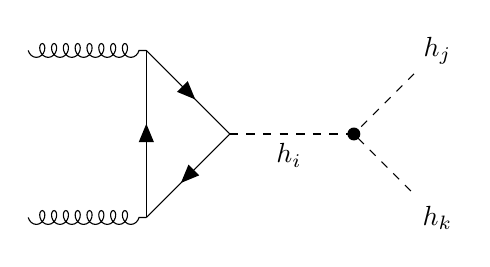
\begin{tikzpicture}
\begin{feynman}
\vertex (i1);
\vertex [right = of i1] (t1);
\vertex [dot][below right =of t1] (t3);
\vertex [below left= of t3] (t2);
\vertex [left = of t2] (i2);
\vertex [right =of t3][dot](h){};
\vertex [above right = of h] (f1){\(h_{j}\)};
\vertex [below right = of h] (f2){\(h_{k}\)};
\diagram* {
(i1) -- [gluon] (t1),
(i2) -- [gluon] (t2),
(t1) -- [fermion](t3) -- [fermion] (t2) -- [fermion](t1),
(t3) -- [scalar,edge label'=\(h_{i}\)] (h),
(f1) -- [scalar] (h) -- [scalar](f2)
};
\end{feynman}
\end{tikzpicture}
\hspace{1cm}
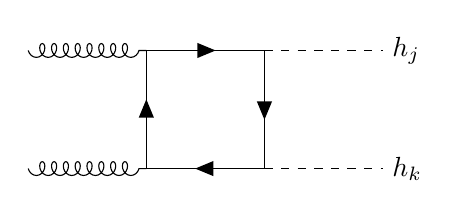
\begin{tikzpicture}
\begin{feynman}
\vertex (i1);
\vertex [ right = of i1] (t1);
\vertex [right = of t1] (t2);
\vertex [below = of t2] (t3);
\vertex [left = of t3] (t4);
\vertex [ left=of t4] (i2);
\vertex [ right =of t2] (f1){\(h_{j}\)};
\vertex [ right=of t3] (f2){\(h_{k}\)};
\diagram* {
(i1) -- [gluon] (t1),
(i2) -- [gluon] (t4),
(t1) -- [fermion](t2) -- [fermion] (t3) -- [fermion](t4) -- [fermion] (t1),
(t2) -- [scalar] (f1),
(t3) -- [scalar] (f2)
};
\end{feynman}
\end{tikzpicture}
\caption[BSM di-Higgs production diagrams]{Feynman diagrams for the production of ${h_{j}h_{k}}$, ${i, j, k = 1, 2, 3}$.}
\label{fig:FeyComp}
\end{center}
\end{figure}


\indent In the limit of ${\theta_{2}\rightarrow{0}}$, which is in agreement with the single Higgs rates, ${h_{3}}$ does not directly couple to SM fermions or vector bosons. The only way to produce ${h_{3}}$ is through ${h_{1}}$ or ${h_{2}}$, with the largest production rate from ${gg\rightarrow h_{2}\rightarrow h_{1}h_{3}}$, figure ~\ref{fig:FeyComp}. For a range of masses ${m_{2}}$ and ${m_{3}}$ the rate of production of ${h_{1}h_{3} \gg h_{1}h_{1}}$, figure ~\ref{fig:CSH6}. \newline

\begin{figure}[h]
\begin{center}
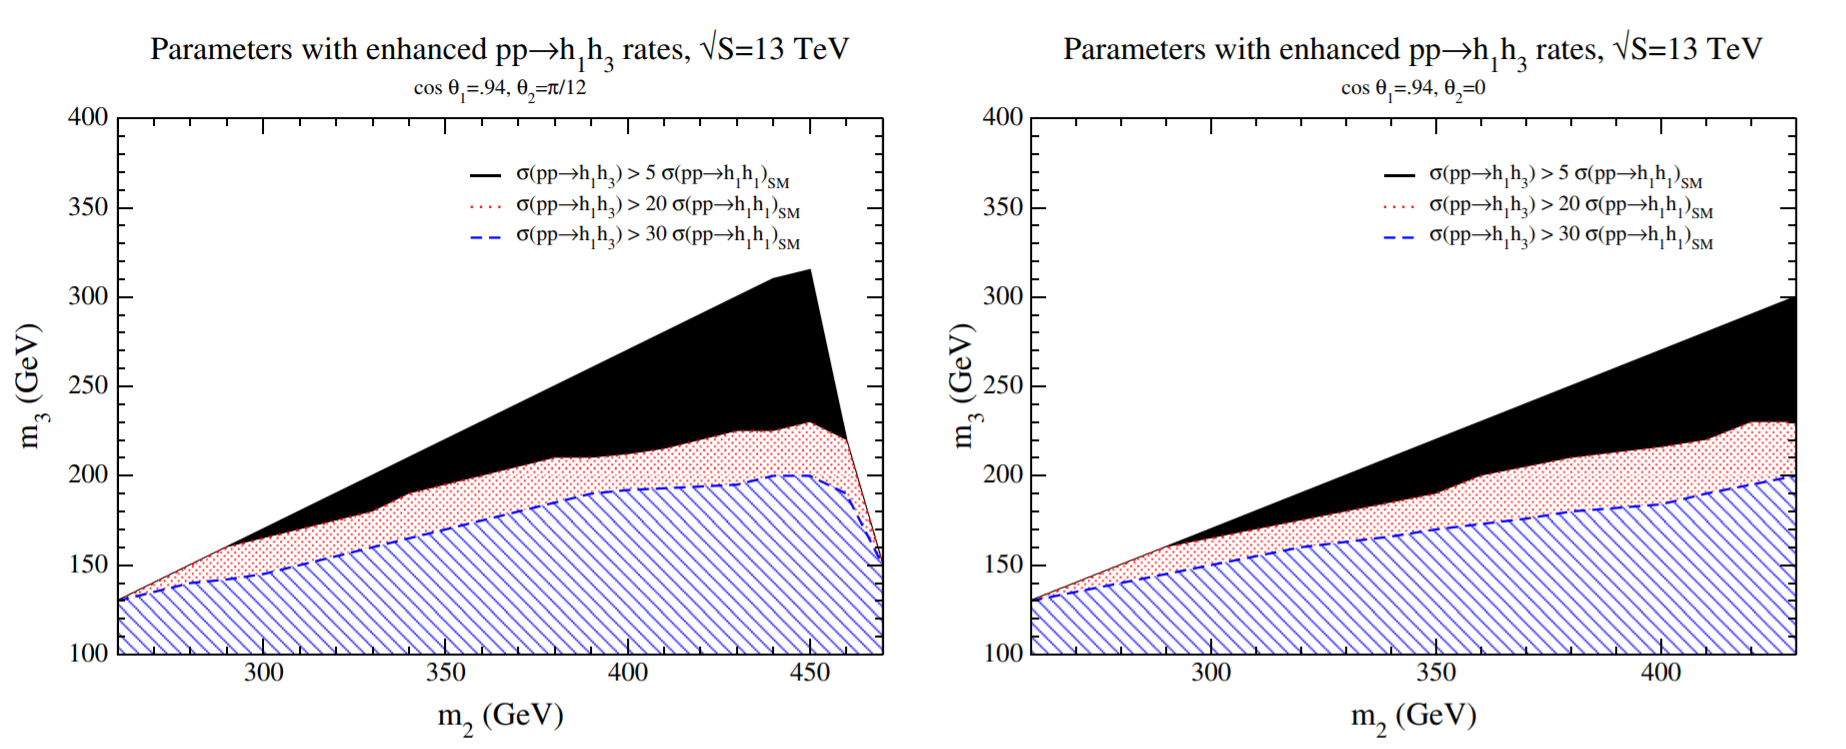
\includegraphics[scale=0.4]{figures/CompHiggsSing_Fig6_2}
\caption[Allowed regions of parameter space with enhanced di-Higgs production]{Regions of parameter space allowed by limits on oblique parameters $S$ $T$ and $U$ from Ref~\cite{deBlas2016}, perturbative unitarity of $2\rightarrow2$ scattering process \cite{PhysRevD.16.1519}, and the minimization of the potential where the rate for ${h_{1}h_{3}}$ production is significantly larger than the SM ${h_{1}h_{1}}$ rate at ${\sqrt{S} = 13 \text{ TeV}}$.}
\label{fig:CSH6}
\end{center}
\end{figure}


The enhancement can be see in the potential where 
\begin{equation}
V \rightarrow \frac{1}{2}\lambda_{211}h_{1}^{2}h_{2} + \frac{1}{2}\lambda_{311}h_{1}^{2}h_{3} + \frac{1}{2}\lambda_{331}h_{1}h_{3}^{2} + \frac{1}{2}\lambda_{321}h_{1}h_{2}h_{3} + . . .
\label{addhiggs}
\end{equation}
So while the SM trilinear Higgs coupling is determined by ${m_{h}}$, with this extension, the coupling is much less constrained. This leads to enhanced values seen in figure \ref{fig:CHS8}. So while this model would definitely show up in SM di-Higgs production, through the first two terms in equation ~\ref{addhiggs}, a search for one SM Higgs and a heavy Higgs would be more sensitive. This is a promising search moving forward but is not the focus of this dissertation.
\begin{figure}[h]
\begin{center}
\includegraphics[scale=0.65]{figures/CompHiggsSing_Fig8}
\caption[Allowed regions of parameter space with enhanced trilinear coupling]{Region of parameter space allowed by limits on oblique parameters, perturbative unitarity and the minimization of the potential where the ${h_{1}h_{1}h_{1}}$ trilinear coupling is greater than 5 times the SM value.}
\label{fig:CHS8}
\end{center}
\end{figure}

\subsection{Real Higgs Singlet Extension}
One simple explanation of an enhanced di-Higgs production rate at the LHC is the addition of a real scalar Higgs singlet, S \cite{Lewis:2017dme}. In this model, S can only interact with the SM through the Higgs field. In the case where there is no ${Z_{2}}$ symmetry, where ${S\rightarrow -S}$ the scalar field S mixes with the SM Higgs boson. If the mass is large enough, it is possible for S to decay to two on-shell SM Higgs Bosons, significantly enhancing the di-Higgs production rate.\newline
\indent The most general potential that can be added is 
\begin{equation}
V(\Phi,S) = -\mu^{2}\Phi^{\dagger}\Phi + \lambda(\Phi^{\dagger}\Phi)^{2} + \frac{a_{1}}{2}\Phi^{\dagger}\Phi S + \frac{a_{2}}{2}\Phi^{\dagger}\Phi S + b_{1}S + \frac{b_{2}}{2}S^{2} + \frac{b_{3}}{3}S^{3} + \frac{b_{4}}{4}S^{4}.
\end{equation}
Where $\Phi$ is ${\phi_{0} = \frac{(h + v)}{\sqrt{2}}}$ and ${<\phi_{0}> = \frac{v}{2}}$, while ${S = s + x}$ where ${x}$ is the vev of S. By shifting the field, it is possible the set ${x = 0}$. After electroweak symmetry breaking the fields mix to give the two mass eigenstates
\begin{equation}
\binom{h_{1}}{h_{2}} = 
\begin{pmatrix}
\cos{\theta} & \sin{\theta}\\
-\sin{\theta} & \cos{\theta}
\end{pmatrix}
\binom{h}{s}
\end{equation}
With ${m_{1} = 125 GeV}$, the free parameters are ${m_{2}, \theta,a_{2},b_{2}}$ and ${b_{4}}$. For di-Higgs production, in the case of ${m_{2}>2m_{1}}$, the important piece of the potential is 
\begin{equation}
V(h_{1}h_{2}) \supset \frac{\lambda_{111}}{3!}h_{1}^{3} + \frac{\lambda_{211}}{3!}h_{2}h_{1}^{2}
\end{equation}
This give an additional resonant double Higgs production diagram , figure ~\ref{fig:FeyRes}, for ${250 \text{ GeV } \leq m_{2}}$.
\begin{figure}[h]
\begin{center}
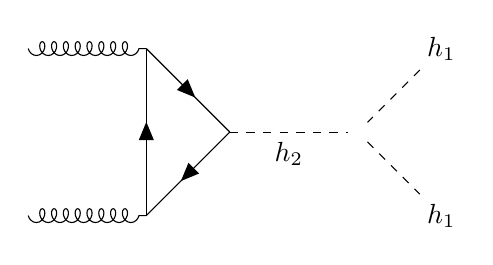
\begin{tikzpicture}
\begin{feynman}
\vertex (i1);
\vertex [right = of i1] (t1);
\vertex [dot][below right =of t1] (t3);
\vertex [below left= of t3] (t2);
\vertex [left = of t2] (i2);
\vertex [right =of t3](h){};
\vertex [above right = of h] (f1){\(h_{1}\)};
\vertex [below right = of h] (f2){\(h_{1}\)};
\diagram* {
(i1) -- [gluon] (t1),
(i2) -- [gluon] (t2),
(t1) -- [fermion](t3) -- [fermion] (t2) -- [fermion](t1),
(t3) -- [scalar,edge label'=\(h_{2}\)] (h),
(f1) -- [scalar] (h) -- [scalar](f2)
};
\end{feynman}
\end{tikzpicture}
\caption[Resonant di-Higgs production diagram]{Feynman diagram for ${h_{2}\rightarrow h_{1}h_{1}}$.}
\label{fig:FeyRes}
\end{center}
\end{figure}

\indent Varying the values of ${b_{4}}$ and ${\sin^{2}{\theta}}$, it is found that the maximum branching ratio (BR) for ${h_{2}\rightarrow h_{1}h_{1}}$ if obtained with ${b_{4} = 4.2, \sin^{2}\theta = 0.12}$. Figure ~\ref{fig:Ian6}, shows the minimum and maximum BR as a function of ${m_{2}}$. The largest BR is when ${m \approx 280 \text{ GeV}}$ at ${BR(h_{2}\rightarrow h_{1}h_{1}) = 0.76}$. This corresponds to an enhancement in di-Higgs production of approximately 30 times the SM cross section.

\begin{figure}[h]
\begin{center}
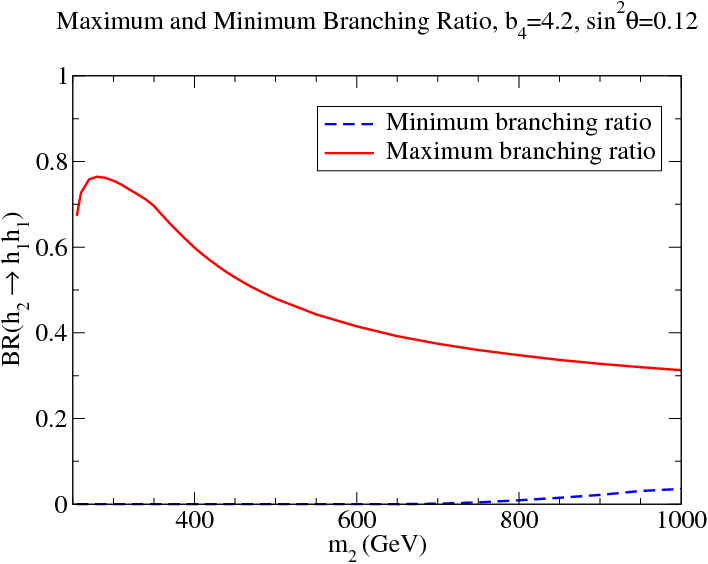
\includegraphics[scale=0.5]{figures/Ian6}
\caption[Allowed branching ratios for resonant di-Higgs production]{Maximum and minimum allowed ${BR(h_{2}\rightarrow h_{1}h_{1})}$ as a function of ${m_{2}}$ for ${b_{4} = 4.2}$ and ${\sin^{2}{\theta} = 0.12}$.}
\label{fig:Ian6}
\end{center}
\end{figure}

\section{Summary}
The SM di-Higgs production rate is an important and achievable measurement for the LHC and HL-LHC. It gives insight to the shape of the Higgs potential through measurement of the trilinear Higgs coupling. It is also a valuable discovery channel for BSM physics, especially for models with an extended Higgs sector, through resonant di-Higgs production. This dissertation will present results for both SM and resonant di-Higgs production.
%%%%%Use this as a filler to get the template working
%%Introduction
\chapter{Experimental Setup}
%ATLAS is a multipurpose detector positioned around one of the 4 primry interaction points of the Large Hadron Collider (LHC) in Geneva, Switzerland. The LHC collides protons at a center of mass energy of 13 TeV, for Run 2, at a rate of approximately 600MHz. 
\section{Hadronic Colliders}
Hadronic colliders use two beams of non-fundamental particles, typically proton-proton or proton-antiproton. These accelerators benefit from the larger mass of the particles when compared to lepton colliders. This results in smaller synchrotron radiation in circular accelerators, as the radiation is inversely proportional to mass. This allows hadronic colliders to have a much larger center of mass energy than leptonic colliders for the same size circular ring. \newline
\indent While hadronic colliders typically have larger collision energies, they also have significantly "messier" collisions. In leptonic colliders, the only final state particles come from the colliding particles. In hadronic colliders, not all of the constituents of the hadrons interact in the hard collision. This leads to many additional particles in the final state. Additionally, each subparticle only carries a portion of the hadron momentum, it is impossible to know the exact initial energy of the collision. 
\section{Overlapping Collisions}
\section{The Large Hadron Collider}
%Source
The Large Hadron Collider (LHC) is a 27 kilometer ring underneath the Franco-Swiss border. The LHC accelerates beams of protons (or ions) to a center of mass energy of up to 13 TeV(5 TeV) in two antiparallel beams around the ring. The particles are then collided at 4 primary interaction points each of which has a dedicated detector: ATLAS, CMS, ALICE, and LHCb.
\subsection{Detector Coordinates}
%Source
Within the ATLAS detector, the interaction point defined the origin of the coordinate system. The z-axis, the longitudinal axis, runs along the beam line, the positive x-axis points toward the center of the LHC ring, and the positive y-axis points toward the surface. The detector is also described in r, ${\eta}$, ${\phi}$ coordinates. With the transverse plane, the plane perpendicular to the beam line, being described by r and ${\phi}$. The radial coordinate, r, describes the distance from the beam line. The azimuthal angle, ${\phi}$, is the angle from the x-axis around the beam line. The final coordinate, ${\eta}$, is referred to pseudorapidity and is defined as ${\eta = -ln(tan(\frac{\theta}{2}))}$. With ${\theta}$ being the angle from the y-axis. The variable ${\Delta{R}=\sqrt{\eta^{2} + \phi^{2}}}$ is used to describe the distance between detector objects.
\section{Detector Overview}
%Source
\begin{figure}[h]
\begin{center}
\includegraphics*[width=0.60\textwidth] {figures/ATLAS_det}%Taken from http://iopscience.iop.org/article/10.1088/1748-0221/3/08/S08003/meta
\caption[The ATLAS detector]{The ATLAS detector}
\label{fig:ATLAS_det}
\end{center}
\end{figure}
The ATLAS detector, Figure~\ref{fig:ATLAS_det} is a general purpose detector and the largest on the LHC.  It is made up of concentric subsystems, each with a specialized task: the inner detector, which is responsible for measuring the charge and momentum of charged particles; the calorimeters, which are responsible for measuring the energy of different electromagnetic and hadronic particles; the muon spectrometer, which measures the momentum of minimum ionizing particles (MIP), like muons; and the magnet system, which is responsible for bending the charged particles in the detector, allowing their charge to be measured. The subdetectors feed into a vast Trigger and Data Acquisition (TDAQ) system that is responsible for selecting collision events with interesting characteristics.

\subsection{The Inner Detector}
%Source Inner detector TDR, I: https://cds.cern.ch/record/331063?ln=en
%Source Inner detector TDR, II: https://cds.cern.ch/record/331064?ln=en
%Source IBL TDR: https://cds.cern.ch/record/1291633?ln=en
\begin{figure}[h]
\begin{center}
\includegraphics*[width=0.60\textwidth] {figures/inner_3D}%Taken from ID TDR
\caption[Cross section of the Inner Detector.]{Cross section of the Inner Detector.}
\label{fig:ID_cs}
\end{center}
\end{figure}
%Tile: https://cds.cern.ch/record/2004868/files/ATL-TILECAL-PROC-2015-002.pdf
%Tile TDR: https://cds.cern.ch/record/331062?ln=en
%LAr TDR: https://cds.cern.ch/record/331061?ln=en
%LAr: https://www.physics.utoronto.ca/~krieger/procs/Krieger_NSS05_Proc.pdf
The inner detector (ID), Figure~\ref{fig:ID_cs}, is the closest system to the beam pipe. It contains 4 separate pieces. In order of distance from the beam pipe: The Insertable B-Layer (IBL), the Pixel Detectors, the Semiconductor Tracker (SCT), and the Transition Radiation Tracker (TRT). These subsystems work together to give charged particle tracking within the pseudorapidity range of ${|\eta| < 2.5}$. The inner detector is surrounded by a 2 T solenoid magnet, section ~\ref{ssec:mag}. The magnetic field causes charged particles to curve as they pass through the ID. The radius and direction of this curve give sign of the charge, positive or negative, along with a momentum measurement of the particle. The other task of the ID is vertexing, or determining if the transient particle came from the interaction point of a slightly displaced point. This is used to identify long lived particles, like bottom or charm quarks. This is discussed further in section ~\ref{ssec:btag}. \linebreak
\indent The IBL is the newest addition to the ID, being installed during the 2016 shutdown. It is place directly outside the beam pipe in order to maintain good vertexing and b tagging in increased pileup environments. In order to facilitate the insertion of the IBL, the beam pipe inner radius was decreased by 4 mm (from 29 mm to 25 mm). The IBL utilizes planar sensors, similar to the Pixel Detector, and 3D sensors, allowing electrons to interact to the bulk of the sensor as opposed to just the surface, and functions as a fourth pixel layer of the Pixel Detector.\linebreak
%Inner detector TDR Fig 3-1
\indent The Pixel Detectors are a network of high granularity, silicon pixels which measure the 2D position of passing charged particles. The silicon pixels are n-doped silicon wafers. A high voltage is applied to the wafer and when a charged particle passes through the silicon an electron hole pair is created. The electron drifts to the electrode and creates a signal that is read out by the electronics.  The Pixel detector barrel is divided into 3 cylindrical layers, the innermost layer is the B-layer, followed by Layer 1 and Layer 2. Each is covered in ${50\mu{m}}$ x ${300\mu{m}}$ silicon pixels. In order to ensure complete coverage, an end cap module is placed on each side of the barrel. The end-caps consist of 4 wheels, each with an inner and outer ring of trapezoid shaped silicon detectors. \linebreak
\indent The SCT is made of a barrel detector and two end-cap detectors. The barrel SCT has 4 cylindrical layers made up of pairs of 6.36 cm x 6.36 cm silicon crystals glued together along one side. The end-cap SCT tracker is made of rings of SCT modules with either silicon or galium arsenide. These rings are arranged into 9 wheels on each side of the barrel.\linebreak
\indent Outside of the silicon detectors lies the TRT. The TRT is a straw detector comprised of 50000, 4mm diameter straws in the barrel and 320000 radial straws in the end-caps. There are 420000 electronic channels, which give a spatial resolution of ${170\mu{m}}$ per straw. The straws are filled with various mixtures of xenon argon, carbon dioxide, tetrafluoromethane and nitrogen gas. When a charged particle passes through the TRT, they ionize the gas. The ionized gas is attracted to the oppositely charged straw and wire and produce a signal that is later amplified and read out. The xenon in the gas mixture allows for accurate particle identification from the transition radiation photon detection.  This gives a good discrimination between electrons and charged pions.

\subsection{Calorimeters}\label{ssec:calo}
%NOTE:::: Add general calo info
Outside of the solenoid magnet lies the calorimetry system. The calorimeters are responsible for measuring the energy of both charged and neutral particles, with the exception of MIPs and non-interacting particles such as neutrinos. The calorimeters can be broken into two distinct pieces, the liquid Argon calorimeter (LAr) and the tile calorimeter. \linebreak
\indent The Liquid Argon (LAr) calorimeter is a sampling calorimeter that is used for electromagnetic calorimetry for the entire range of acceptance (${|\eta{}|<4.8}$). It is also used for hadronic calorimetry for higher pseudorapidity ${1.4<|\eta{}|<4.8}$ In the central "barrel" of the calorimeter (${|\eta{}| < 1.4}$), is made up of 1024 lead-stainless-steel converters with copper-polyimde multilayer readout boards. The pates and readouts are arranged in an "accordion-shaped" geometry, Fig XXX. This allows for complete azimuthal coverage with no gaps, giving a constant electromagnetic energy resolution. In between the accordion layers, liquid argon is used as the active medium. The system is enclosed in a cryostat to maintain the temperature of the detector. The LAr barrel is divided radially into 4 sampling layers that are read out with a granularity of 0.1x0.1 ${\eta}$x${\phi}$ which are referred to as Trigger Towers. The granularity of the layers can be found in table XXXXX (LAR TDR table 1-2). The layer closest to the beamline is the Presampler. This layer sits inside of the cryostat and is responsible for  correcting for the energy loss in front of the calorimeter (the same is done in the endcap). Inside the cryostat, there are 3 additional layers, Fig XXXX. The thickness of the layers is often described in terms of radiation lengths ${\Xi_{0}}$. Where a radiation length is the distance a electron travels before it loses approximately 1/2 of it's energy to photon emission.  The front layer has a thickness of ${4.3\Xi_{0}}$, followed by the middle layer with a thickness of ${16\Xi_{0}}$ and the back layer of thickness ${2\Xi_{0}}$. Since the middle layer is the thickest, the bulk of the energy is absorbed in that layer. \linebreak 
\indent Forward from the barrel, there are two electromagnetic endcap (EMEC) wheels with a similar accordion structure to the barrel. One covering ${1.4 < |\eta{}| < 2.5}$ and one from ${2.5 < |\eta{}| < 3.2}$ Outside of the EMEC is the Hadronic endcap (HEC). This is also a copper-LAr sampling calorimeter. It has a simpler parallel plate design. Finishing out the LAr calorimeter is the Forward Calorimeter (FCal), which is contained in the endcap cryostat. This calorimeter is in the very forward region of the detector. In this region, the particle flux is very high, so a dense calorimeter is necessary to avoid energy leaking into other pieces of the detector. There are 3 layers in the FCAL, the first is made of copper and the other two are made of tungsten. They are matrices of metal with concentric tubes filled with Argon, see Fig XXXXX. TDR fig 1-9. \linebreak
\indent In the central region ${|\eta{}|<1.7}$, the tile calorimeter (TileCal) is responsible for the hadronic calorimetry. The TileCal is a sampling calorimeter with alternating iron plate absorbers and plastic scintillating tiles, the orientation can be seen in Fig XXXX (https://cds.cern.ch/record/2004868/files/ATL-TILECAL-PROC-2015-002.pdf, fig 2) . It has a fixed central barrel and 2 extended barrel sections that can be moved. The TileCal has a depth of ${7.4\lambda{}}$, where ${\lambda{}}$ is the nuclear interaction length, the mean distance a hadronic particle travels before it undergoes an inelastic interaction. The readout has the same granularity as the LAr trigger towers (0.1x0.1)
\subsection{Muon Detectors}
%Figure of muon cutaway: https://www.researchgate.net/figure/4-Cut-away-view-of-the-ATLAS-muon-system-from-Ref-3_fig10_254469099
%muon tdr: http://atlas.web.cern.ch/Atlas/GROUPS/MUON/TDR/pdf_final/mTDR.pdf
To detect muons, ATLAS uses four different technologies. For precision energy and position measurements, monitored drift tubes (MDT) and cathode strip chambers (CSC) are used. The CSCs are used in regions of high flux, where the MDTs are not suitable.  For the muon trigger system, a fast system is needed to keep up with the high collision rate of the LHC. In the central region, resistive plate chambers (RPC) are used, while in the forward region, where flux is higher, thin gap chambers (TGC) are used. The muon system, much like the ID utilize a magnetic field to determine the charge of passing particles. The magnet system is further discussed in Section~\ref{ssec:mag}.\linebreak
\indent The MDTs are made up of 6 parallel layers of cylindrical aluminum drift tubes with a tungsten-rhenium wires. The drift tubes are filled with a mixture of argon, nitrogen and methane. The tubes are assembled on a support of spacer and they are monitored for deformation by a built-in optical system, hence the \textbf{monitored} drift tubes. \linebreak
\indent While the MDTs are very good at precision measurements. However, they are not appropriate in areas whith the high rate counts (${> 200 Hz/cm^{2}}$) sue to their large diameter and high operating pressure. This is the case for the first layer of muon measurement with pseudorapidities of ${|\eta{}|>2.0}$. For this region, CSCs are the spectrometer of choice. CSCs are multiwire proportional chambers with a cathode strip readout. This gives good single and two track resolution in this high rate region.\linebreak
\indent In the barrel region, the muon trigger system employs RPCs, a low occupancy chamber with fast response. RPCs are gaseous parallel-plate detectors of Bakelite. The system can operate in two modes, avalanche and streamer.  In streamer mode, a large potential across the plates generates a discharge around the ionizing particle. For avalanche mode, a smaller potential difference and large signal amplification in the electornics allows for increased rate capability.\linebreak
%http://citeseerx.ist.psu.edu/viewdoc/download?doi=10.1.1.664.2817&rep=rep1&type=pdf
\indent Finally, in the end-cap of ATLAS, TGCs provide 2 important components. For the trigger system, TGCs have good timing resolution compared to the MDTs and can deal with a rate of up to 100 ${KHz/cm^{2}}$. For measurement, TGCs provide the azimuthal coordinate to compliment the bending coordinate from the MDTs. The TGCs are made up of anode wires and graphite cathodes in between layers of fiberglass laminate. 
\subsection{Magnet System}\label{ssec:mag}
%https://cds.cern.ch/record/338080?ln=en


\subsection{Trigger System}
\subsubsection{L1 Trigger}
\subsubsection{High Level Trigger}
\section{Simulation}





%%%%%Use this as a filler to get the template working
%%Introduction
\chapter{Simulation and Event Reconstruction}

\section{Simulation}
In order to draw conclusion from ATLAS data, it is necessary to compare to theoretical predictions. For particle collisions, it is not practical to create exact predictions, especially including detector effects such as resolution. To get the best estimate of these effects, ATLAS uses the Monte Carlo (MC) method to simulate data. This is done in multiple steps as illustrated by figure ~\ref{fig:eventsim}. \newline

\begin{figure}[h]
\begin{center}
\includegraphics*[width=0.70\textwidth] {figures/event_simulation}
\caption{Pictorial representation of how an event is generated \cite{Wanotayaroj:2242196}}
\label{fig:eventsim}
\end{center}
\end{figure}


\indent At the energies at the LHC, collisions usually do not involve entire protons. Instead, they involve constituents known as partons. Protons, while often described as two up quarks and a down quark, contain a sea of gluons. This sea of gluons also creates many virtual quark-antiquark pairs. The up and down quarks are the outer, or valance, quarks. These valance quarks are the primary role players in shallow inelastic interactions. At the LHC, the collision energies are sufficient for deep inelastic scattering, where the affects of the internal quarks and gluons are non-trivial. This internal structure of the proton is described  by a Parton Distribution Function (PDF), figure ~\ref{fig:pdf}. A PDF shows the probability density of finding a parton carrying a momentum fraction ${x}$ at a squared energy scale. %(http://www.scholarpedia.org/article/Introduction_to_Parton_Distribution_Functions)
\newline

\begin{figure}[h]
\begin{center}
\includegraphics*[width=0.65\textwidth] {figures/pdf.jpg}
\caption{The bands are ${x}$ times the unpolarized parton distributions
${f(x)}$ (where ${f = u_{v}, d_{v}, \bar{u}, \bar{d}, s \simeq{} \bar{s}, c = \bar{c}, b = \bar{b}, g}$) obtained in NNLO NNPDF3.0
global analysis at scales ${\mu^{2} = 10  GeV^{2}}$
(a) and ${\mu^{2} = 100  GeV^{2}}$ (b), with
${\alpha_{s}(M^{2}_{Z}) = 0.118}$.}
\label{fig:pdf}
\end{center}
\end{figure}


\indent The hard scattering process can be described using Feynman diagrams. These diagrams are a pictorial representation of amplitudes. These amplitudes go into calculating the matrix elements (ME) various interactions. In the event generation, these MEs are calculated to a specified order in perturbation theory. Common examples are leading order(LO), next-to-leading order(NLO) , and so on. The higher the order of the calculation, the more accurate the predictions. However, higher orders can be extremely hard to theoretically calculate. Often restricting the level of the event generator. \newline
\indent  After the ME generator, the hard partons are used as the inputs to the Parton Shower (PS) calculation. The PS calculation takes the hard scattering process from the event generator and calculates the parton shower. In addition to calculating the parton shower, the PS also calculates additional hard radiation processes not included in the base interaction. Colored particles can spontaneously emit gluons. These gluons, in turn, create either more gluons, or quark-antiquark pairs. This can happen either before (ISR) or after (FSR) the hard scattering process. Along with the ISR and FSR emittance, the PS generator can also describes the hadronization and subsequent decay of the hadrons into the final state particles. The precision of the PS generators are described similarly to the ME, with their contributions coming in as leading log (LL), next-to-leading-log (NLL), etc. for the parton showering process. \newline
\indent Finally, once the PS generator is complete, it is necessary to model the interactions of the final state particles as they pass through the ATLAS detector. ATLAS uses GEANT4  to handle this propagation\cite{geant4}. \newline
\indent The final result of the MC event generation is a set of simulated data that resembles actual data from the p-p collisions in the ATLAS detector. 
\section{Particle Identification}
For all events, either MC or actual collision data, it is important to be able to identify and reconstruct the underlying physics event. In particle collisions, the energy from the final state particles is deposited in the various subdetectors within ATLAS. These energy deposits must be translated to physically meaningful objects. This is the task of the event reconstruction, to use the ATLAS detector to recreate the final state particles for any given interaction. For this analysis, the final state particles present in the signal events are a lepton, either an electron or a muon; a neutrino, in the from of missing transverse energy; two light flavor quarks; and two b quarks. Each of these particles has a particular signal in each of the subdetectors, figure ~\ref{fig:crossSec}.

\begin{figure}[h]
\begin{center}
\includegraphics*[width=0.70\textwidth] {figures/layers}
\caption{Event Cross Section in a computer generated image of the ATLAS detector \cite{Pequenao:1096081}}
\label{fig:crossSec}
\end{center}
\end{figure}


\subsection{Electrons}
Electrons are reconstructed by fitting a track using the Inner Detector and matching this track to an energy cluster in the EM calorimeter\cite{Tarna:2286383}. As an electron passes through the EM calorimeter, it produces Bremsstahlung radiation photons. These photons then convert back to electron-positron pairs and the process repeats. This shower of electrons, positrons, and photons give the signature energy cluster in the calorimeter. Particles with the required Inner Detector track and matching EM energy cluster are selected as electron candidates.\newline
\indent Electron identification algorithms are applied to these electron candidates. These algorithms separate prompt, isolated electron candidates from backgrounds such as converted photons and misidentified jets. The electron identification algorithm is a multivariate likelihood discriminant using shower shape, track and track-to-cluster matching discriminating variables. There are three identification working points for electron identification: Loose, Medium, and Tight. Where the operating points wit higher background rejection are a subset of electron candidates with lower background rejection.\newline
\subsection{Muons}
The Muon Spectrometer specializes in muon detection and precision momentum measurement. Unsurprisingly, this makes the Muon Spectrometer (MS) a vital part of muon identification, but it is not the only subdetector used. The Inner Detector is also has an important part in reconstructing muons. In ATLAS, muon reconstruction is performed independently in the Inner Detector and the MS. The information is then combined to for the muon tracks. In the Inner Detector, the muons are reconstructed similarly to any other charged particle.\newline
\indent In the MS, the reconstruction looks for a hit pattern within each chamber to form segments \cite{Aad:2016jkr}. The MDT segments are combined using a straight-line fit. Segments in the CSCs are combined using a combinatorial search in the ${\eta}$ and ${\phi}$ planes. \newline
\indent Muon candidates are built by fitting together hits from segments in different layers. A combinatorial search, using segments in the middle layer as seeds, is performed. The inner and outer layers are then used as seeds as the search is extended. A minimum of 2 segments are required to build a track. It is possible for a segment to be included in multiple tracks, an overlap removal algorithm selects the best assigned track or can allow for a segment to be shared between two tracks. A global ${\chi^{2}}$ fit is performed on the hits of each track. If the ${\chi^{2}}$ of the fit passes a selection criteria, the track is accepted.\newline
\indent The information from the Inner Detector and the MS are then combined to give a muon signature. The combination method depends on the information available. The main method used is the Combined Muon reconstruction, where track reconstruction is performed in the Inner Detector and MS independently. Most of these muons are reconstructed using an ''outside-in" reconstruction. This  means tracks in the MS are extrapolated inward and matched to an Inner Detector track. \newline
\subsection{Jets}
Quarks very quickly undergo hadronization, with only the top quark decaying before hadronizing. This makes it impossible to measure a singular quark. Instead, collections of hadrons are formed and these are what deposit energy in the ATLAS detector. These collections of energy are called jets and can be made from various detector object. In this analysis in particular, two different types of jets are used: calo-jets, jets constructed from energy deposited in the calorimeters; and track-jets, jets constructed from tracks in the Inner Detector. \newline
\indent Since a jet is not a physical object, rather a collection of energy deposits, there are many ways to define a jet. Two important characteristics of any jet algorithm are Infrared (IR) Safety and Collinear (CL) Safety. For a jet algorithm to be IR Safe, the addition or subtraction of a soft jet will not change the jet collection. A jet algorithm is CL Safe if splitting or merging high transverse momentum particles does not change the jet collection. Figure \ref{fig:IR_CL} illustrates both IR and CL Safety.

\begin{figure}[h]
\begin{center}
\includegraphics*[width=0.70\textwidth] {figures/IR_CL_safe}
\caption{Illustration of the infrared sensitivity of a cursory designed jet algorithm (top). Illustration of the product of a collinear unsafe jet algorithm. A collinear splitting changes the number of jets (bottom). \cite{Isildak:2013kfa}.}
\label{fig:IR_CL}
\end{center}
\end{figure}

\indent Some examples of jet algorithms are visualized in figure ~\ref{fig:jetalgo}. For this analysis, the ${\textrm{anti-}k_{t}}$ algorithm is selected. In addition to being IR and CL safe, the ${\textrm{anti-}k_{t}}$ algorithm gives roughly circular jets. This makes calculating the energy density much easier than non-circular jets. The ${\textrm{anti-}k_{t}}$ algorithm has a radius parameter R. R acts as a cutoff radius for energy clustering and is not strictly a radius. The track-jets used in the analysis have R = 0.2, while the R = 0.4 and R = 1.0 calo-jets are used. \newline 

\begin{figure}[h]
\begin{center}
\includegraphics*[width=0.70\textwidth] {figures/jetalgo}
\caption{A sample parton-level event, together with many random soft
``ghosts", clustered with four different jets algorithms, illustrating the ``active" catchment areas of
the resulting hard jets\cite{Cacciari:2008gp}.}
\label{fig:jetalgo}
\end{center}
\end{figure}

\subsection{b Tagging}\label{ssec:btag}
B-Hadrons, composite particles that contain b quarks, travel a small distance before they decay. This means the track from the decay products can be traced back to the point at which the b-hadron decays, called the secondary, or displaced, vertex, figure ~\ref{fig:bjets} . This displaced vertex is used to tag jets that are likely to come from b quarks through b-tagging algorithms.\newline
\indent In this analysis, the MV2c10 is used to tag b-jets \cite{ATL-PHYS-PUB-2016-012}. MV2 is a multivariate discriminant that combines 3 b-tagging algorithms. The c10 signifies a 10\% c-jet fraction in the background training sample. The three algorithms that are used as inputs to the MV2 discriminant are: an impact parameter-based algorithm, an inclusive secondary vertex reconstruction algorithm, and a decay chain multi-vertex reconstruction algorithm. For this analysis, the 85\% fixed-cut working point is used for b-jet identification.\newline

\begin{figure}[h]
\begin{center}
\includegraphics*[width=0.70\textwidth] {figures/bjet}
\caption{Schmatic view of the tracks in a b-jet \cite{HanssonAdrian:1397942}.}
\label{fig:bjets}
\end{center}
\end{figure}

\subsection{Missing Transverse Momentum}
Neutrinos do not interact with the detector as they pass through. This means they cannot be measured like the other particles. In order to measure neutrinos, ATLAS relies on the conservation of momentum. As previously mentioned, the exact collision energy is unknown, as each partons does not carry a consistent fraction of the proton energy. However, in the transverse plane, the plane perpendicular to the beam line, the total momentum is known exactly. Before the collision, there is zero momentum in the transverse plane. After the collision, this must also be true. This implies the vector summation of all objects should have zero momentum in the transverse plane. Any imbalance in this is referred to as  Missing Transverse Momentum (\met). The \met{} is constructed as the negative vector sum of all reconstructed objects with an additional soft term reconstructed from detector signal objects not associated with any object\cite{ATL-PHYS-PUB-2015-027}. \newline
\indent The \met{} vector is a vector in the transverse plane, meaning it does not directly correspond to a neutrino. Additional information is needed to exactly reconstruct a neutrino. In this analysis, a Higgs mass constraint is used to supply the direction of the signal neutrino. \newline


%%%%Use this as a filler to get the template working
%%Introduction
\chapter{Analysis}
\section{Motivation}
\section{Data and Monte Carlo Samples}
\section{Object Selection}
\subsection{Electrons}
\subsection{Muons}
\subsection{Jets}
\subsection{Missing Transverse Energy}
\section{Event Selection}
\section{Background Determination}
\subsection{Data Driven QCD}
\section{Uncertainties}
\section{Results}
\section{Conclusion}


%%%%%Use this as a filler to get the template working
%%Introduction
\chapter{Conclusion}
\label{chap:conc}
A search for resonant and non-resonant Higgs boson pair production in the ${b\overline{b}WW^{*}}$ decay mode is done in the ${b\overline{b}l\nu qq}$ final state using $pp$ collision data with an integrated luminosity of 36.1 fb\textsuperscript{-1} collected at ${\sqrt{s}}$ = 13 TeV by the ATLAS detector at the LHC. No excess of events over the background only expectation is found. Limits are set on resonant and non-resonant production. \newline
\indent In addition to the complete analyses presented in this dissertation, an complimentary event reconstruction is presented. This new fully boosted analysis offers roughly a factor of two increase in sensitivity for the same dataset and is a promising addition to the ${HH\rightarrow b\overline{b}WW^{*}\rightarrow b\overline{b}l\nu qq}$ analysis for the full Run I analysis. 

%\begin{appendices}
\appendix
%\include{sanityChecks}
%\appendix
%\include{signalContamination}
%\end{appendices}
%\end{linenumbers}

%% List of contributors - print here or after the Bibliography.
%%\PrintAtlasContribute{0.30}
%%\clearpage
%
%%-------------------------------------------------------------------------------
%%%%%Use this as a filler to get the template working
%%Introduction
\chapter{Introduction}
The Standard Model (SM) is the culmination of more than a century of work. The first piece added to the puzzle was the electron, discovered in 1891. Since then, 24 other particles have been discovered, with the final piece, the Higgs Boson, being added in 2012. Since it was theorized, the SM has held up to rigorous experimentation and remains an unbeaten theory of fundamental matter and forces. Even though the SM is widely successful, it fails to explain all observed phenomena. Gravity, neutrino masses, dark matter, along with other observations, all lacking explanation within the SM. The remaining task is to probe the extremes of the SM to either more precisely measure the parameters or to find its limit.
%Include this is a search for BSM production
\section{The Standard Model}
The Standard Model defines the basic building blocks of matter and force and the interactions between them. Normal matter that we interact with on a daily basis is made of protons, neutrons, and electrons. Electrons are a fundamental particle, called a lepton, meaning they are not made of smaller constituents. However, protons and neutrons are not fundamental particles. They are a composite of up and down quarks, two more fundamental particles. The protons are made of 2 ups and a down and the neutrons are made of two downs and an up. Leptons and quarks are both different types of fermions. \linebreak
\indent Fermions are spin-${\frac{1}{2}}$ particles that make up all matter in the SM. The fermions can be broken down into 3 "generations". Where a generation contains two quarks, one with electric charge ${+\frac{2}{3}}$ and one with electric charge ${-\frac{1}{3}}$, one electrically charged lepton, charge -1, and one electrically neutral lepton. The quarks have an additional color charge, of which there are 3 charges. This is additional quantum number associated with the strong force. In all, this gives 12 fermions. \linebreak 

\begin{table}[h]
\begin{center}
\footnotesize
\begin{tabular}[h]{|c||c|c|c|c|}
\hline
 & Particle & Spin & Charge & Mass \\
\hline\hline
Quarks &&&&\\
\hline
u type &u& & &${2.4^{+0.6}_{-0.4} MeV}$\\
 &c&${\frac{1}{2}}$&${\frac{2}{3}}$&${1.28\pm{0.03} GeV}$\\
 &t& & &${173.1\pm{0.6} GeV}$\\
\hline
d type & d& & & ${4.7^{+0.5}_{-0.4} MeV}$\\
 & s & ${\frac{1}{2}}$ & ${-\frac{1}{3}}$ & ${96^{+8}_{-4} MeV}$\\
 & b & & & ${4.18^{+0.04}_{-0.03} GeV}$\\
\hline\hline
Leptons &&&&\\
\hline
e family & e & ${\frac{1}{2}}$ & -1 &${0.5109989461\pm{}0.000000003 MeV}$\\
 & ${\nu_{e}}$ & & 0 & ${< 2 eV}$\\
 \hline
${\mu}$ family & ${\mu}$ & ${\frac{1}{2}}$ & -1 &${105.6583745\pm{}0.0000024 MeV}$\\
 & ${\nu_{\mu}}$ & & 0 & ${< 2 eV}$\\
 \hline
${\tau}$ family & ${\tau}$ & ${\frac{1}{2}}$ & -1 &${1776.86\pm{}0.12 GeV}$\\
 & ${\nu_{\tau}}$ & & 0 & ${< 2 eV}$\\
 \hline\hline
 Bosons &&&&\\
 \hline
 Vector & ${\gamma}$ & 1 & 0 & ${< 10^{-18} eV}$\\
 & ${g}$ & 1 & 0 & ${0}$\\
 & ${W}$ & 1 & ${\pm}$ & ${80.385\pm{}0.0015 GeV}$\\
 & ${Z}$ & 1 & 0 & ${91.1876\pm{}0.0021 GeV}$\\
 \hline
 Scalar & H & 0& 0 & ${125.09\pm{}0.21\pm{}0.11 GeV}$\\
 \hline
\end{tabular}
\caption{Particles of the Standard Model (ref XXX (ian or PDG))}
\label{tab:SM}
\end{center}
\end{table}

\indent Gauge bosons are spin-${1}$ particles responsible for carrying the fundamental forces in the standard model. There are 12 physical gauge boson. The photon ${\gamma}$ is a massless, charge neutral force carrier for the electromagnetic force. The nuclear forces are carried by 3 massive gauge bosons. A chargeless Z boson and two charged W bosons, ${Q = \pm 1}$. Together, these 4 bosons control the electroweak interactions in the standard model. The remaining 8 bosons are the gluons, the force carriers for the strong nuclear interaction. Gluons are massless, electrically neutral particles that have two color charges. There is a gluon for each combination of the three color charges, giving the 8 total gluons. \linebreak
\indent The remaining piece of the standard is the Higgs Boson. The Higgs boson is a massive Scalar, spin-${0}$, chargeless boson. The Higgs boson is responsible for giving mass to the massive electoweak bosons through electroweak symmetry breaking. The particles and their properties are in Table ~\ref{tab:SM}\linebreak
\subsection{Interactions}
The SM is governed by three different types of interactions. For leptons, the overarching theory is quantum electrodynamics (QED). QED describes how particles behave under electroweak interactions. This can be broken down further into the electromagnetic interaction and the weak interaction. The electromagnetic interaction defines the interaction of electrically charged particles with photons. The fundamental diagram for the electromagnetic interaction is electron-positron annihilation ~\ref{Fey:e-p}. Where an electron and a positron collide and produce two photons. This can also be reversed, two photons interact and produce an electron-positron pair. The strength of this interaction is the electrical charge e. \linebreak

\begin{figure}[h]

\begin{center}
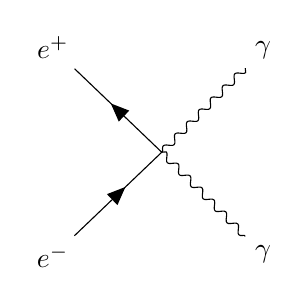
\begin{tikzpicture}
\begin{feynman}
\vertex (c) ;
\vertex [below left =of c] (i1){\(e^{-}\)};
\vertex [above left=of c] (i2) {\(e^{+}\)};
\vertex [below right=of c] (f1){\(\gamma\)};
\vertex [above right= of c] (f2){\(\gamma\)};
\diagram* {
(i1) -- [fermion] (c) -- [fermion] (i2) ,
(f1) -- [photon] (c)-- [photon] (f2)
};
\end{feynman}
\end{tikzpicture}
\caption{Electron-Positron Annihilation}
\label{Fey:e-p}
\end{center}
\end{figure}

\indent The weak interaction defines the interaction of particles under the weak isospin quantum number. There are two copies of each of every fermion, a left and a right-handed chirality version. Particle with a right-handed chirality have a weak isospin T = 0. These particles exist as singlets and do not interact with the weak force. Left-handed particles have a weak isospin T =  ${\frac{1}{2}}$. These particles live as doublets as illustrated in table ~\ref{tab:chiral}. For these particles, the third component of the weak isospin T\textsubscript{3}, ${+\frac{1}{2}}$ for up-type quarks and charged leptons and ${-\frac{1}{2}}$ for down-type quarks and neutral leptons. Under weak interactions, particles with ${T_{3} = +\frac{1}{2}}$ always transform into particles with ${T_{3} = -\frac{1}{2}}$, or vice versa.\linebreak

\begin{table}[h]
\begin{center}
\def\arraystretch{1.5}
\begin{tabular}[h]{|c|c|}
\hline
Left Handed Fermions, ${T = \frac{1}{2}, T_{3} = \pm\frac{1}{2}}$ & Right Handed Fermions, ${T = 0, T_{3} = 0}$\\
\hline\hline
${\binom{u}{d}}$, ${\binom{c}{s}}$, ${\binom{t}{b}}$, ${\binom{e}{\nu_{e}}}$, ${\binom{\mu}{\nu_{\mu}}}$, ${\binom{\tau}{\nu_{\tau}}}$ & u, d, c, s, t, b, e, ${\nu_{e}}$, ${\mu}$, ${\nu_{\mu}}$, ${\tau}$, ${\nu_{\tau}}$ \\
\hline
\end{tabular}
\caption{Particles of the Standard Model (ref XXX (ian or PDG))}
\label{tab:chiral}
\end{center}
\end{table}


 \indent The remaining piece of the weak interaction is the W boson. The W has an isospin of T = 1. This gives three option for the third component of isospin, ${T_{3} = +1, 0, -1}$ which give the W\textsuperscript{+}, the W\textsuperscript{0}, and the W\textsuperscript{-}. W\textsuperscript{0} will be discussed more in ~\ref{ssec:Higgs}. The ${W^{\pm}}$ either raise or lower the ${T_{3}}$ of the fermions. ~\ref{Fig:weak_dia} is an example of a weak interaction.\linebreak

\begin{figure}[h]
\begin{center}

\begin{tikzpicture}
\begin{feynman}
\vertex (i1){\(e^{-}\)};
\vertex [right =of i1] (c);
\vertex [right=of c] (f1) {\(\nu_{e}\)};
\vertex [below right=of c] (f2){\(W^{-}\)};
\diagram* {
(i1) -- [fermion] (c),
(f2) -- [boson] (c)-- [fermion] (f1)
};
\end{feynman}
\end{tikzpicture}
\caption{electron emitting an electron neutrino and a W Boson}
\label{Fig:weak_dia}
\end{center}
\end{figure}

%Here, write about mixing and electroweak interaction?
%Also need to talk briefly about QCD
%Need to talk about b-quarks specifically.

%\begin{equation}
%Y_{W} = 2(Q - T_{3})
%\end{equation}


\indent %Need to talk about couplings and decays more in depth here
\subsection{The Higgs Mechanism and Higgs Boson}
\label{ssec:Higgs}
%Start with need massless gauge bosons to fufill local gauge invariance. So we have W 1,2,3, and b. explain the mixing and the  break the symmetry to give the W+- Z and photon. Give math to explain this?? Show how this gives rise to a new boson, the higgs. 
QED is a gauge invariant theory. This means the Lagrangian that describes the system is invariant under local gauge transformations. For the electroweak theory, this is the electroweak symmetry. To satisfy this symmetry, the bosons must be massless. However, the electroweak bosons in the standard model, the ${W^{\pm}}$ the ${Z}$ and the ${\gamma}$ are not all massless. This means that the electroweak symmetry must be broken by something.\linebreak

\begin{figure}[h]
\begin{center}
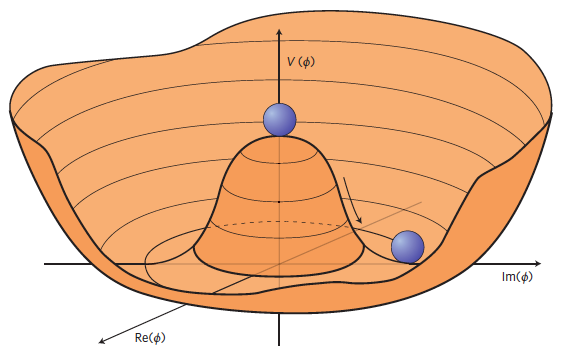
\includegraphics[scale=0.65]{figures/higgspotential}
\caption{The Higgs potential (from http://cds.cern.ch/record/1638469/plots) }
\label{Fig:higgspot}
\end{center}
\end{figure}

\indent In QED, the five gauge bosons are ${W^{i}_{\mu}, i = 1,2,3}$ and ${B_{\mu}}$. These bosons couple to a complex scalar Higgs doublet, ${\Phi \equiv \binom{\phi^{+}}{\phi^{0}}}$. This doublet has a scalar potential.
\begin{equation}
V(\Phi) = \mu^{2}|\Phi^{\dagger}\Phi| + \lambda(|\Phi^{\dagger}\Phi|)^{2}
\end{equation}
Where ${\mu^{2} < 0}$. This gives the Mexican hat shaped potential seen in figure ~\ref{Fig:higgspot}, with a minimum energy at 
\begin{equation}
\langle \phi \rangle = \sqrt{-\frac{\mu^{2}}{2\lambda}}\equiv \frac{\nu}{\sqrt{2}}
\end{equation}
called the vacuum expectation value (VEV) of ${\phi}$. The choice of the direction of fluctuation is arbitrary but can be chosen such that


 
\begin{equation}
\phi_{0} = \frac{1}{\sqrt{2}} \binom{0}{\nu}
\end{equation}
After the direction is chosen and the only remaining piece is the scalar field h(x), giving 
\begin{equation}
\phi(x) = \phi_{0} + h(x)
\end{equation}
The doublet can now be described by 
\begin{equation}
\Phi = \frac{1}{sqrt{2}} \binom{0}{v+h(x)}
\end{equation}
The Higgs field couples to the gauge bosons as 
\begin{equation}
(\frac{g}{2}\overrightarrow{\tau}\cdot \overrightarrow{W} + \frac{g'}{2}B)\phi_{0}
\end{equation}
Where ${\overrightarrow{\tau}}$ are the Pauli matrices, ${\overrightarrow{W}}$ are ${W_{1,2,3}}$ and g, g' are the coupling constants. The result of the coupling is the acquisition of mass by three eigenstates of the bosons, 
\begin{equation}
\begin{split}
W^{\pm} = \frac{1}{\sqrt{2}}(W^{1}_{\mu} \mp iW^{2}_{\mu})\\
Z^{\mu} = \frac{-g'B_{\mu} + gW^{3}_{\mu}}{\sqrt{g^{2} + g'^{2}}}\\
A^{\mu} = \frac{gB_{\mu} + g'W^{3}_{\mu}}{\sqrt{g^{2} + g'^{2}}}
\end{split}
\end{equation}
These four eigenstates are the bosons we observe in the standard model. With Masses
\begin{equation}
\begin{split}
M^{2}_{W} = \frac{1}{4}g^{2}\nu^{2} \\
M^{2}_{Z} = \frac{1}{4}(g^{2} + g'^{2})\nu^{2} \\
M_{A} = 0
\end{split}
\end{equation}
Through the mixing that occurs in the spontaneous electroweak symmetry breaking gives mass to the standard model Gauge Bosons while leaving the photon massless. However, for this to occur, an additional scalar field, the Higgs Field, is required.\linebreak
\indent The Higgs Boson is an excitation in the scalar Higgs field predicted in 1964. The decay mechanism of this massive boson was predicted by Peter Higgs, allowing for the decay products to be measured. Giving a way to prove the existence of the scalar Higgs field. In 2012, a Higgs like scalar boson was discovered at the LHC by the ATLAS and CMS experiments with a mass of 125GeV/c\textsuperscript{2} (ref XXX https://arxiv.org/abs/1207.7214). Since the discovery, many measurements have been made of this Higgs Boson to compare it to the standard model Higgs Boson. So far, the Higgs Boson has held up to these tests. The Higgs Boson has spin-parity J\textsuperscript{P} = 0\textsuperscript{+} 
(ref XXX %https://www.sciencedirect.com/science/article/pii/S0370269313006527?via%3Dihub)
, decays to bb (https://www.sciencedirect.com/science/article/pii/S0370269318307056), ${\gamma\gamma, \tau\tau}$,(ref XXX https://arxiv.org/abs/1811.08856) WW and ZZ have been measured with appropriate signal strengths, and no significant deviations have been observed in any Run 2 analyses. However, there are still many parameters of the Higgs Boson that still need measured. One of which is the triple Higgs coupling.
%Do I want to include more about the higgs discovery. 

%%\clearpage
%%-------------------------------------------------------------------------------
%
%
%%%-------------------------------------------------------------------------------
%\input{ATLASdetector}
%%\clearpage
%%-------------------------------------------------------------------------------
%
%%%-------------------------------------------------------------------------------
%\input{TriggerData}
%%\clearpage
%%-------------------------------------------------------------------------------
%
%
%%%-------------------------------------------------------------------------------
%\input{Simulation}
%%\clearpage
%%-------------------------------------------------------------------------------
%
%
%%%-------------------------------------------------------------------------------
%\input{Reconstruction}
%%\clearpage
%%-------------------------------------------------------------------------------
%
%
%%-------------------------------------------------------------------------------
%\input{SignalRegions}
%%\clearpage
%%%-------------------------------------------------------------------------------
%
%
%%%-------------------------------------------------------------------------------
%\input{Background}
%%\clearpage
%%-------------------------------------------------------------------------------
%
%
%%%-------------------------------------------------------------------------------
%\input{Systematics}
%%\clearpage
%%-------------------------------------------------------------------------------
%
%
%%%-------------------------------------------------------------------------------
%\input{Results}
%\clearpage
%%-------------------------------------------------------------------------------
%
%%
%%% All figures and tables should appear before the summary and conclusion.
%%% The package placeins provides the macro \FloatBarrier to achieve this.
%%% \FloatBarrier
%%
%%
%%-------------------------------------------------------------------------------
%\input{Conclusions}
%%\clearpage
%%%-------------------------------------------------------------------------------
%%
%%-------------------------------------------------------------------------------
%%%-------------------------------------------------------------------------------
%%
%
%
%%The \texttt{atlaslatex} package contains the acknowledgements that were valid 
%%at the time of the release you are using.
%%These can be found in the \texttt{acknowledgements} subdirectory.
%%When your ATLAS paper or PUB/CONF note is ready to be published,
%%download the latest set of acknowledgements from:\\
%%\url{https://twiki.cern.ch/twiki/bin/view/AtlasProtected/PubComAcknowledgements}
%
%%The supporting notes for the analysis should also contain a list of contributors.
%%This information should usually be included in \texttt{mydocument-metadata.tex}.
%%The list should be printed either here or before the table of contents.
%
%
%%-------------------------------------------------------------------------------
%%\clearpage
%%\appendix
%%\part*{Appendix}
%%\addcontentsline{toc}{part}{Appendix}
%%%-------------------------------------------------------------------------------
%%
%%In a paper, an appendix is used for technical details that would otherwise disturb the flow of the paper.
%%Such an appendix should be printed before the Bibliography.
%
%
%-------------------------------------------------------------------------------
% If you use biblatex and either biber or bibtex to process the bibliography
% just say \printbibliography here

\printbibliography
%\printbibliography[title={REFERENCES CITED},heading=bibintoc]
%\bibliographystyle{atlasBibStyleWithTitle}
%\bibliography{CONF}
% If you want to use the traditional BibTeX you need to use the syntax below.
%\bibliographystyle{bibtex/bst/atlasBibStyleWoTitle}
%\bibliography{atlas-document,bibtex/bib/ATLAS}
%-------------------------------------------------------------------------------

%-------------------------------------------------------------------------------
% Print the list of contributors to the analysis
% The argument gives the fraction of the text width used for the names
%-------------------------------------------------------------------------------
%\clearpage
%\PrintAtlasContribute{0.30}

%%-------------------------------------------------------------------------------


%\clearpage


%\appendix
%\input{auxMaterial}
%\appendix
%%\part*{Auxiliary material}
%%\addcontentsline{toc}{part}{Auxiliary material}
%%-------------------------------------------------------------------------------

%In an ATLAS paper, auxiliary plots and tables that are supposed to be made public 
%should be collected in an appendix that has the title \enquote{Auxiliary material}.
%This appendix should be printed after the Bibliography.
%At the end of the paper approval procedure, this information can be split into a separate document
%-- see \texttt{atlas-auxmat.tex}.
%
%In an ATLAS note, use the appendices to include all the technical details of your work
%that are relevant for the ATLAS Collaboration only (e.g.\ dataset details, software release used).
%This information should be printed after the Bibliography.
\end{runninglinenumbers}
\end{document}
